\documentclass[letterpaper,12pt]{article}
\usepackage{tabularx} % extra features for tabular environment
\usepackage{amsmath}  % improve math presentation
\usepackage{float}
\usepackage{pdfpages}
\usepackage{cite}
\usepackage{multicol}
\usepackage{graphicx} % takes care of graphic including machinery
\graphicspath{ {./figures/} }
%\usepackage[margin=1in,letterpaper]{geometry} % decreases margins

\usepackage[final]{hyperref} % adds hyperlinks inside the generated pdf file
\hypersetup{
    colorlinks=true,       % false: boxed links; true: colored links
    linkcolor=blue,        % color of internal links
    citecolor=blue,        % color of links to bibliography
    filecolor=magenta,     % color of file links
    urlcolor =blue         
}
\usepackage[margin = 1in,headsep=0.5cm,headheight=2cm,letterpaper]{geometry} 
\usepackage{subcaption}

\usepackage{fancyhdr}

\usepackage{listings}
\usepackage{color}

\definecolor{dkgreen}{rgb}{0,0.6,0}
\definecolor{gray}{rgb}{0.5,0.5,0.5}
\definecolor{mauve}{rgb}{0.58,0,0.82}

\lstset{frame=tb,
  language=Python,
  aboveskip=3mm,
  belowskip=3mm,
  showstringspaces=false,
  columns=flexible,
  basicstyle={\small\ttfamily},
  numbers=none,
  numberstyle=\tiny\color{gray},
  keywordstyle=\color{blue},
  commentstyle=\color{dkgreen},
  stringstyle=\color{mauve},
  breaklines=true,
  breakatwhitespace=true,
  tabsize=3
}




\pagestyle{fancy}
\lhead{Intern: Ahmet Akman 2442366  \\ Supervisor: Dr. Johannes Zierenberg}
%\rhead{Date: \today \\ Duration: 19.07.22-21.08.22} 
%\cfoot{center of the footer!}
\renewcommand{\headrulewidth}{0.1pt}

\title{

\includegraphics[width=17cm]{odtu.png} \\

\includegraphics[width=4cm]{eee.png} \\
\vspace*{0.5in}
\textbf{EE400 Summer Practice Report}
\vspace*{0.25in}
}

\author{Intern: Ahmet Akman 2442366\\
Supervisor: Dr. Johannes Zierenberg\\
Supervisor Contact: \href{mailto: johannes.zierenberg@ds.mpg.de}{ johannes.zierenberg@ds.mpg.de. }-\href{tel:+495515176475}{+495515176475}\\
Assigned Faculty Member: Prof.Dr. Engin Tuncer\\
Institution Name: Max Planck Institute for Dynamics and Self-Organization\\
Start date:03.07.2023 || End date: 22.09.2023\\
        \vspace*{0.25in} \\
        Electrical and Electronics Engineering Department\\
        \textbf{Middle East Technical University}\\
        Ankara, Turkey
       } \date{\today}


\begin{document}

\bibliographystyle{plain}

%\thispagestyle{empty}
%\includepdf[pages=-]{coverpage_signed.pdf}


\maketitle

\newpage
\tableofcontents
\newpage
%\begin{abstract}
%abstract
%\end{abstract}
\section{Introduction}
\section{About Institution}
\subsection{Institution Name}
Max Planck Institute for Dynamics and Self-Organization.
\subsection{Institution Location}
Max Planck Institute for Dynamics and Self-Organization
Am Faßberg 17
37077 Göttingen
Germany
\subsection{General Description}
The Max Planck Institute for Dynamics and Self-Organization, located in Göttingen, Germany, is a prominent research institution primarily focused on the investigation of complex non-equilibrium systems, particularly within the fields of physics and biology. Its historical roots trace back to 1911 when Ludwig Prandtl initiated the establishment of a Kaiser Wilhelm Institute dedicated to the study of aerodynamics and hydrodynamics. This initial effort led to the formation of the Aeronautische Versuchsanstalt in 1915, which later evolved into the Kaiser Wilhelm Institute for Flow Research in 1924. In 1948, it became a part of the Max Planck Society. In 2003, it underwent a name change and became the Max Planck Institute for Dynamics and Self-Organization. Presently, it stands as one of the 80 institutes under the auspices of the Max Planck Society, contributing significantly to the understanding of intricate dynamic systems.

\subsection{Organization Structure}
The organization structure of the institute is given in Figure \ref{organization}. I was part of the group led by Prof.Dr. Viola Priesemann which is indicated as italic on \ref{organization}.

\begin{figure}[htbp] \centering{
    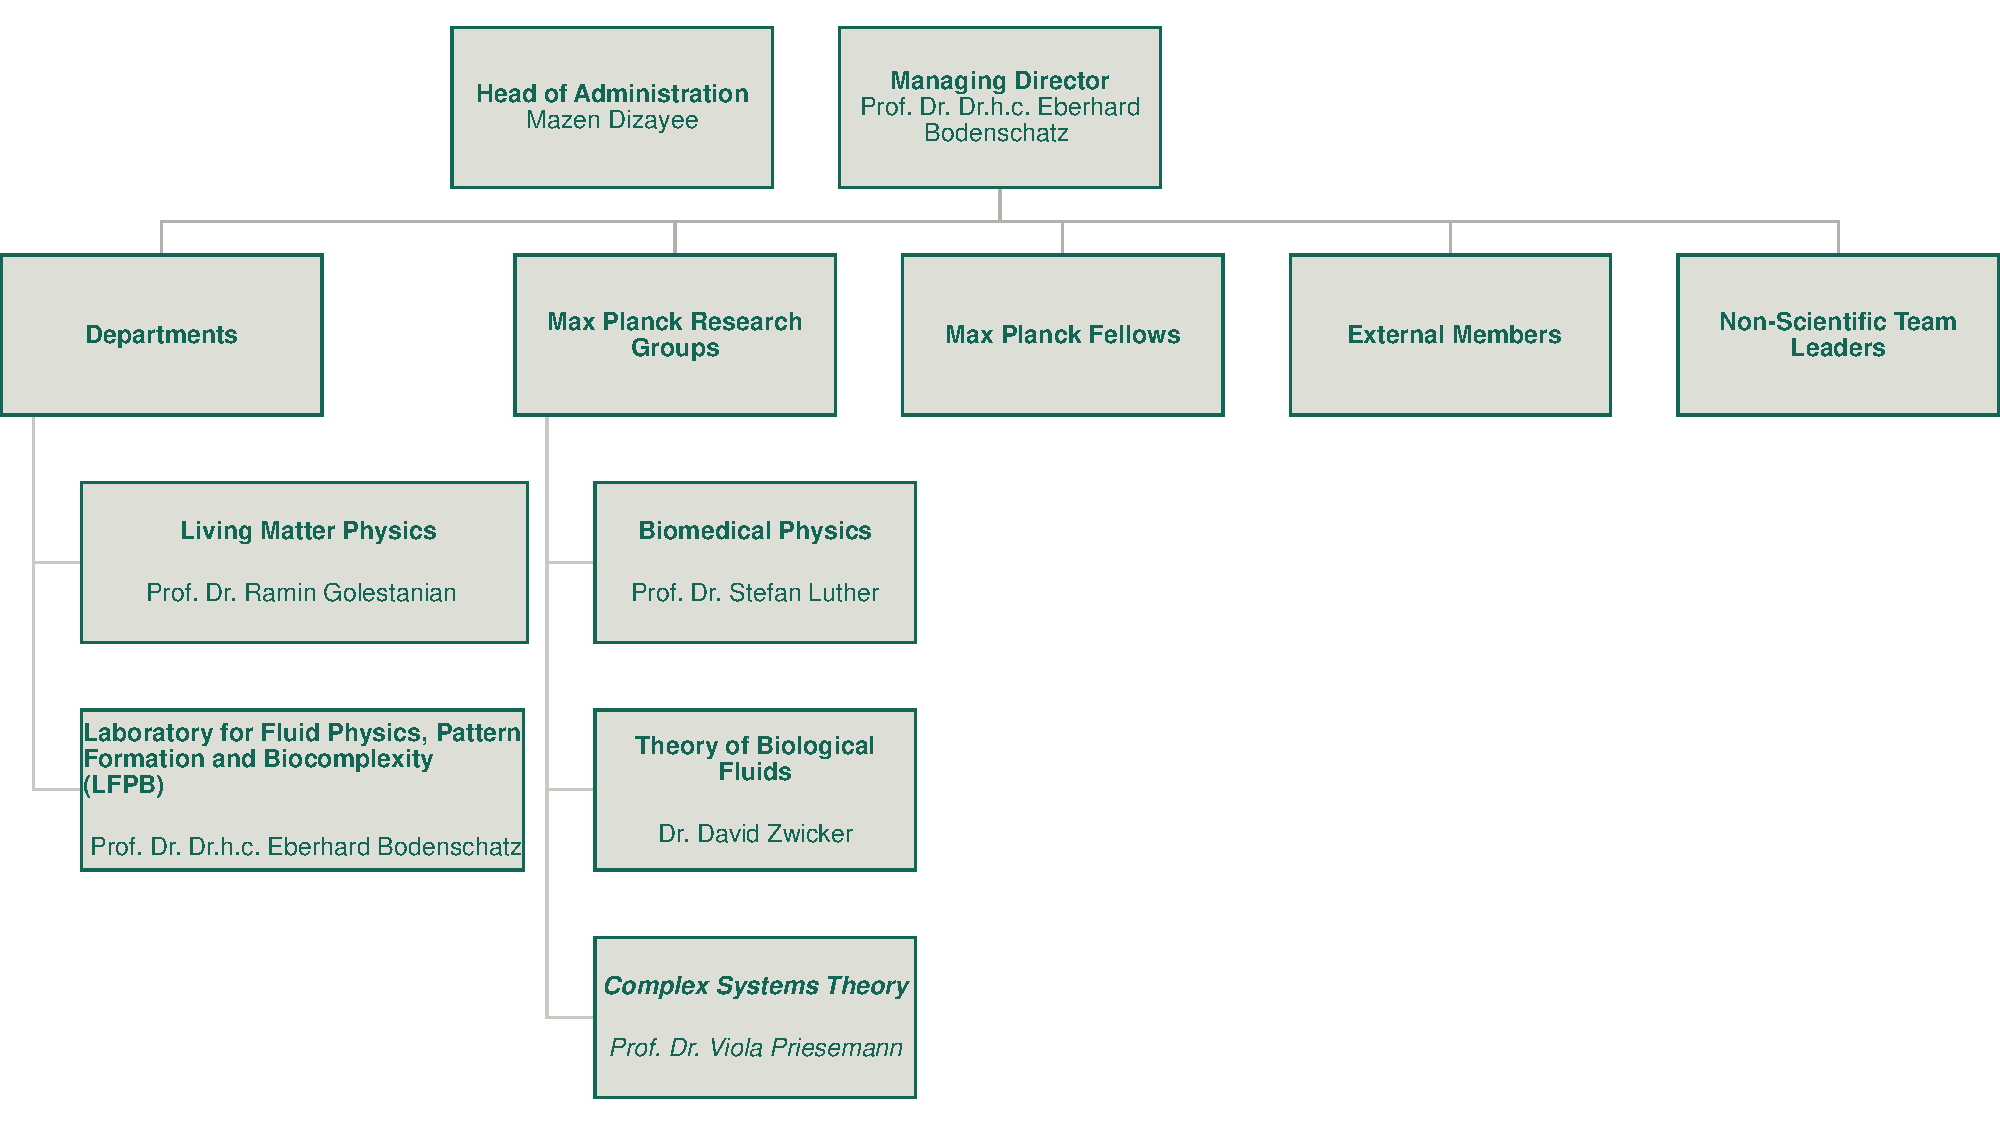
\includegraphics[width=\linewidth]{OrgChartMPIDS.pdf}}
    \caption{Basic organizational structure of MPI-DS.}
    \label{organization}
\end{figure}

\section{Project Background and Motivation}
The research project for the internship is constructed upon the following set of previous research. In the field of neuroscience \cite{CHAOS}, initiated the idea of inhibition is a necessary part of a neuronal network for stability of the network. Then, the impactful paper \cite{brunel} explained the dynamics of a sparsely connected random network with fixed parameters. Also, the role of inhibition was similar to the \cite{CHAOS}. The phases of the network through these dynamics are also stated. These states can be summarized as follows also givein in Figure \ref{brunel_fig}. Synchronous regular (SR) is the state where the whole network is blinking in a synchronized way. So, the neurons are synchronized with each other, exciting each other together, and regular activity is observed. Synchronous irregular (SI) is the state where the individual neurons show irregular activity, but the global activity is still regular. Therefore, the rate of the random network is still blinking in some sense. SI-fast and SI-slow characterize this as two different dynamical states. The asynchronous irregular state is the desired stable state where both the individual (per-neuron) and global activity show irregularity, that is, to small average overall activity not-blinking global network. \cite{brunel} has been considered as a guiding baseline in the field, and many other network descriptions built upon this idea, including inhibition as a factor for stability. It is important to note that the \cite{brunel} employs a fixed set of parameters on a completely randomly connected network.

\begin{figure}[htbp]
    \centering
    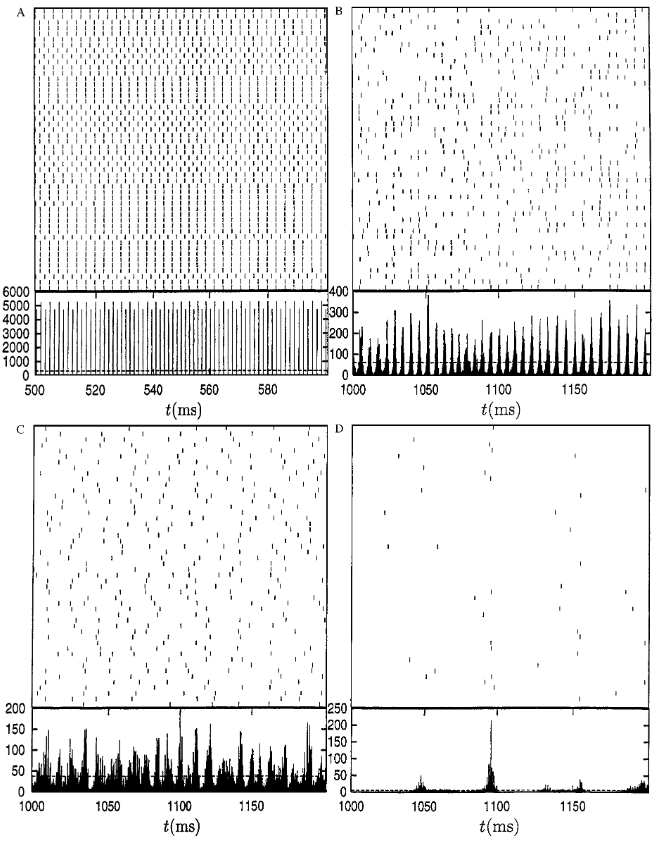
\includegraphics[width = 0.5\textwidth]{brunel.png}
    \caption{The states of the network. (A) Synchronous Irregular. (B) Synchronous Irregular-fast. (C) Asynchronous Irregular. (D) Synchronous Irregular-slow.}
    \label{brunel_fig}
\end{figure} 

\subsection{Hypothesis}

In neurobiology, one can classify the neurons as excitatory and inhibitory. A typical excitatory neuron is called a pyramidal neuron, whereas there are more than 20 mainstream types of inhibitory neurons. The idea is that the role of inhibition might be something other than just stabilizing the network. So, we hypothesize that only excitatory networks can be stable. To achieve the stability, the structural connectivity of the network should be reconsidered. \cite{2Dstructure} describes the 2D layered structure of the cortical networks in the brain. 

\section{Project Description}
The project is built upon the hypothesized idea frame. First, the tools for the project are determined. For simulation implementation, Python programming language and a brain simulator package called Brian2 \cite{brian2} are used. The simulations run on the HPC (High-performance computing cluster.), which is set to be used with the industry standard SGE (Sun Grid Engine). The project timeline aligns with the report format presented in this document. 

\subsection{2D Connectivity}
The 2D locality of the network is somewhat intuitive as the neurons in the cortical networks have a higher probability of connection to nearby neurons. In order to model this phenomenon, first, the $N$ number of neurons is randomly located in the $1 by 1$ area. Then, according to the "smallest distance" between each pair, the probability map is constructed by zero-mean Gaussian. Figure \ref{prob_map} gives an example probability map for $N = $. In this formulation, the outdegree $K$ of the neurons is fixed. That is to say, one neuron has a fixed number of outgoing connections. In other words, one axon has a fixed number of synapses. According to the probability map, the connection assignment process is conveyed as picking $K$ number of neuron $j$'s to connect neuron $i$ without replacement. A sample is given in Figure \ref{connectionmap}.

\begin{figure}[htbp]
    \centering
    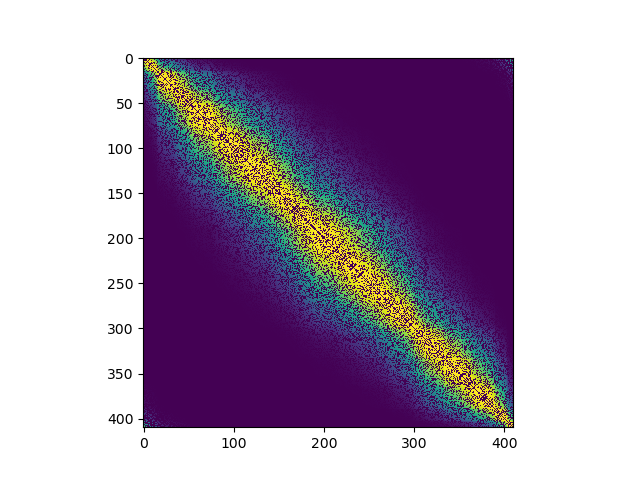
\includegraphics[width = 0.75\textwidth]{prob_map.png}
    \caption{Sample probability map for $N = 512$}
    \label{prob_map}
\end{figure} 

\begin{figure}[htbp]
    \centering
    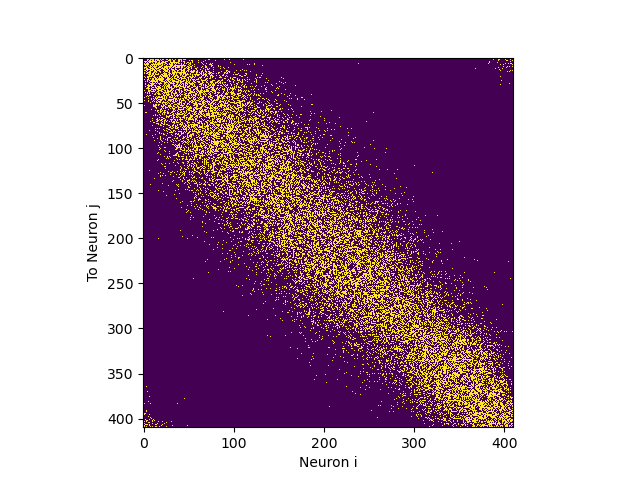
\includegraphics[width = 0.75\textwidth]{connections.png}
    \caption{Sample connection map for $N = 512$}
    \label{connectionmap}
\end{figure} 
Also, the connections for one neuron are illustrated in Figure \ref{neuron_network} as a part of the whole network for $N=10000$ and $K=100$, which is the standard network size through the rest of the study.

\begin{figure}[htbp] \centering{
    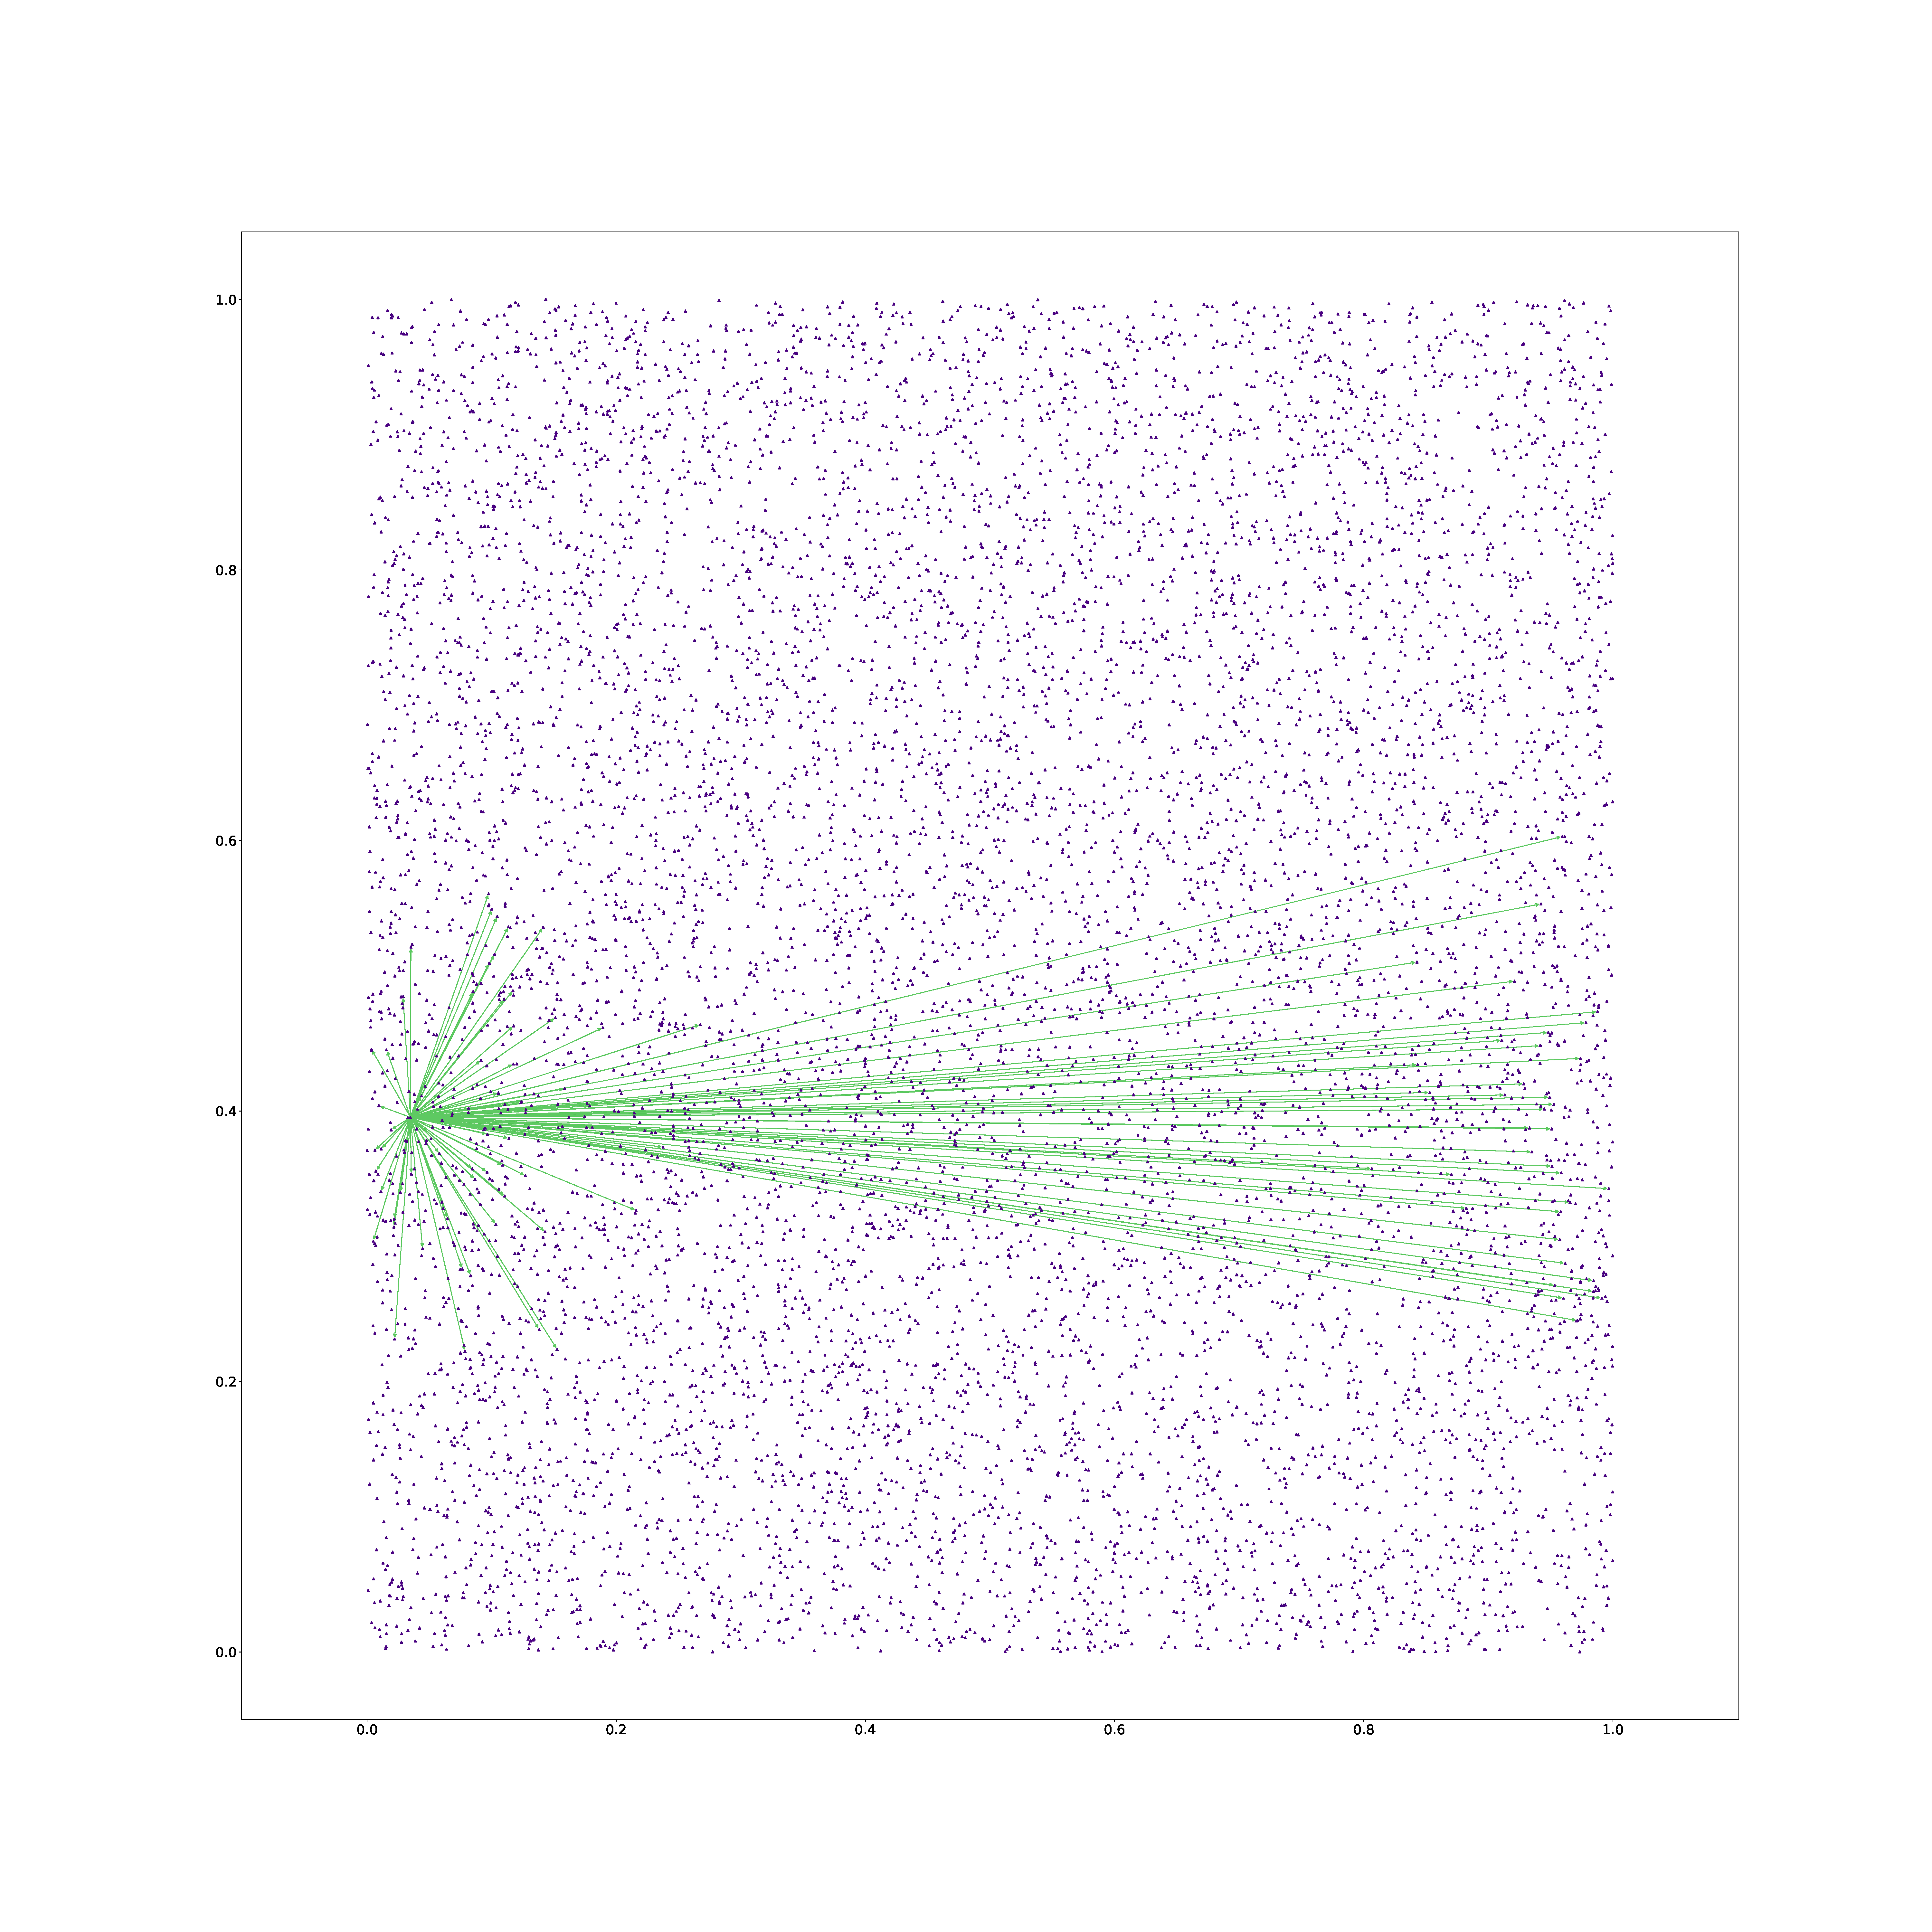
\includegraphics[width=\linewidth]{neuron_network.pdf}}
    \caption{Connections of a neuron on the bigger network size.}
    \label{neuron_network}
\end{figure}


There are two important points that should be stated. First, the "smallest distance" is being calculated as if the 2D plane has periodic boundary conditions, creating 3D torus structure. Second, as the outdegree is fixed the $\sigma$ value, which is the standard deviation of the Gaussian function has two limitations. One dependent on the system size, the other one is dependent on the outdegree. Since the periodic boundary conditions apply, larger $\sigma$ loses its effectiveness. On the other hand, as the $\sigma$ goes smaller and smaller it becomes impossible distinguish between two different values because of the fixed number of selections, so one can not go more local in that sense. To be able to illustrate this situation the Figure \ref{effectivesigma}. On x axis the $\sigma$ value for the probability map is ranged. On y axis the $effective \text{ } \sigma$ which is the average distance of the connected neurons, is given. This plot allowed us to choose a small and useful enough $\sigma$ value. 
\begin{figure}[htbp] \centering{
    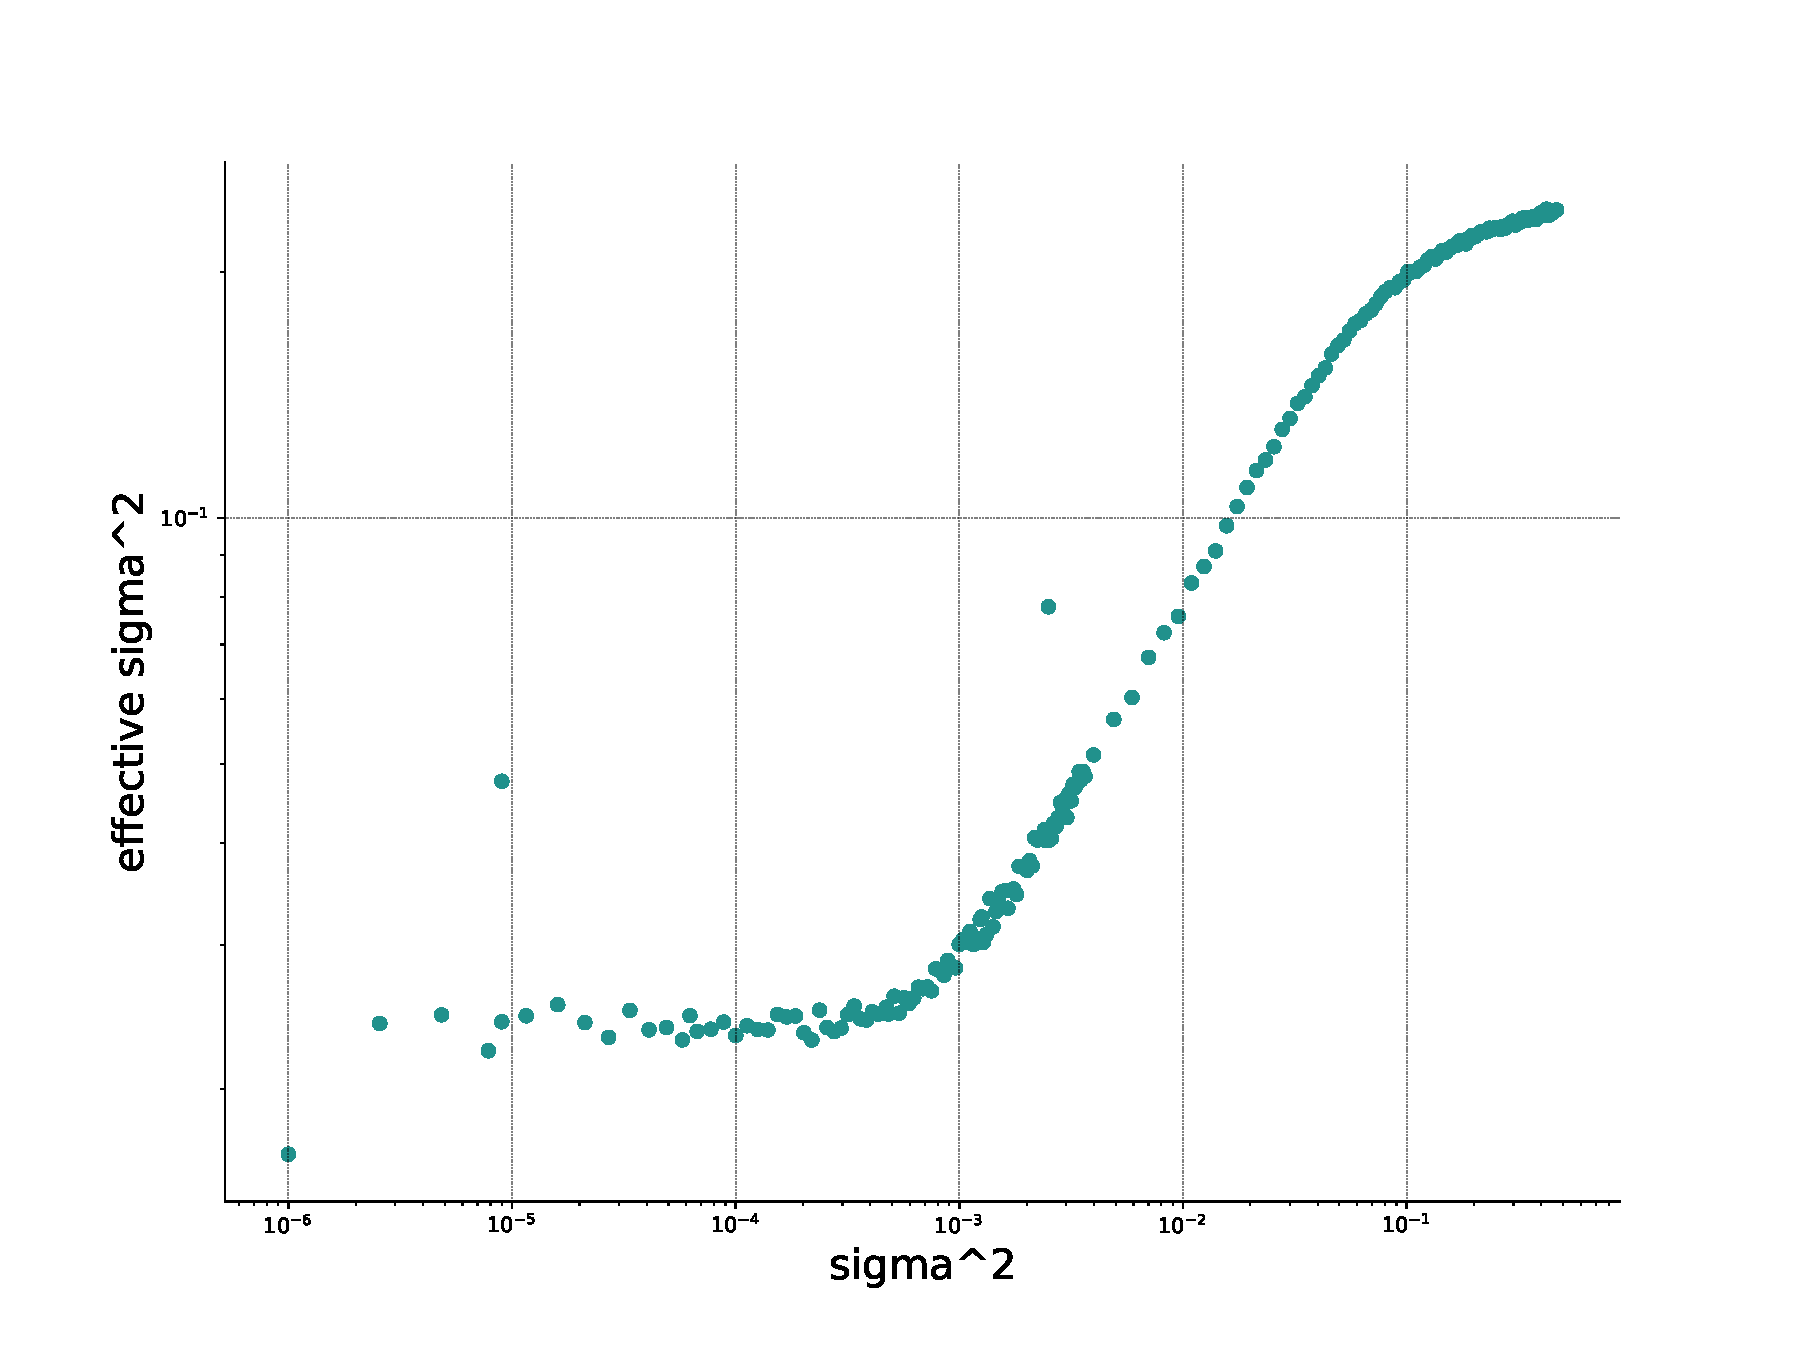
\includegraphics[width=\linewidth]{K_rec100_N_10000_K_rec100_N_10000.pdf}}
    \caption{effective $\sigma ^2$ vs $\sigma ^2$.}
    \label{effectivesigma}
\end{figure}



\subsection{Baseline}
First, the simulations that form our basis are done via setting a  
\subsection{Homeostastatic Regulation}
\subsection{Future Projection on the Project}

\section{Project Implementation and Results}
\subsection{Baseline Results}
\subsection{Homeostatic Regulation Results}

\section{Conclusion}
\section{References}
\bibliography{refs/cite}

\section{Appendix}

\end{document}

%%%%%%%%%%%%%%%%%%%%%%   EXAMPLE TABLE   %%%%%%%%%%%%%%%%%%%%%%%%%%%%%%%%
\begin{table}[H]
\begin{center}
    \caption{Resistance reading by color code convention.}
    \vspace{2mm}
    \begin{tabular}{||c | c | c||} 
        \hline
        Color Order & Value & Tolerance \\ [0.5ex] 
        \hline\hline
        Brown / Black / Red / Gold & 1k\( \Omega \) & \( \% \) 5  \\ 
        \hline
        Yellow / Violet / Red / Gold & 4.7k\( \Omega \) & \( \% \) 5   \\
        \hline
        Brown / Grey / Orange / Gold & 18k\( \Omega \) & \( \% \) 5  \\ [1ex] 
        \hline
    \end{tabular}
\end{center}
\end{table}


%%%%%%%%%%%%%%%%%%%%%%   EXAMPLE IMAGE   %%%%%%%%%%%%%%%%%%%%%%%%%%%%%%%%
\begin{figure}[H]
\centering
\includegraphics[width = 1\textwidth]{5.png}
\caption{Circuit schematic for step 5}
\end{figure} 

%%%%%%%%%%%%%%%%%%%%%%   EXAMPLE IMAGE FROM PDF   %%%%%%%%%%%%%%%%%%%%%%%%%%%%%%%%
\begin{figure}[H] \centering{
    \includegraphics[scale=0.25]{2a_plot.pdf}}
    \caption{Experiment 2}
\end{figure}
